We are going to get an idea on how various applications of dimensionality reduction look like and how they behave.

\subsection{Improve computational performance}

This one is the most obvious.
We are going to find examples of projects / use cases where the performance is greatly improved without affecting the models performance.

Maybe the MNIST dataset?

\clearpage





\subsection{Improve model performance}

A little less obvious.
Find a model that performs better after dimensionality reduction.
Talk about the curse of dimensionality and overfitting a model.

Maybe try my research project?

\clearpage





\subsection{Visualisation}

Showcase how data can be represented in different ways.

Maybe see 33c3 (\href{https://www.youtube.com/watch?v=-YpwsdRKt8Q}{Reverse Engineering von Spiegel-Online (33c3)})

Should look something like this:

\begin{figure}[h]
  \centering
  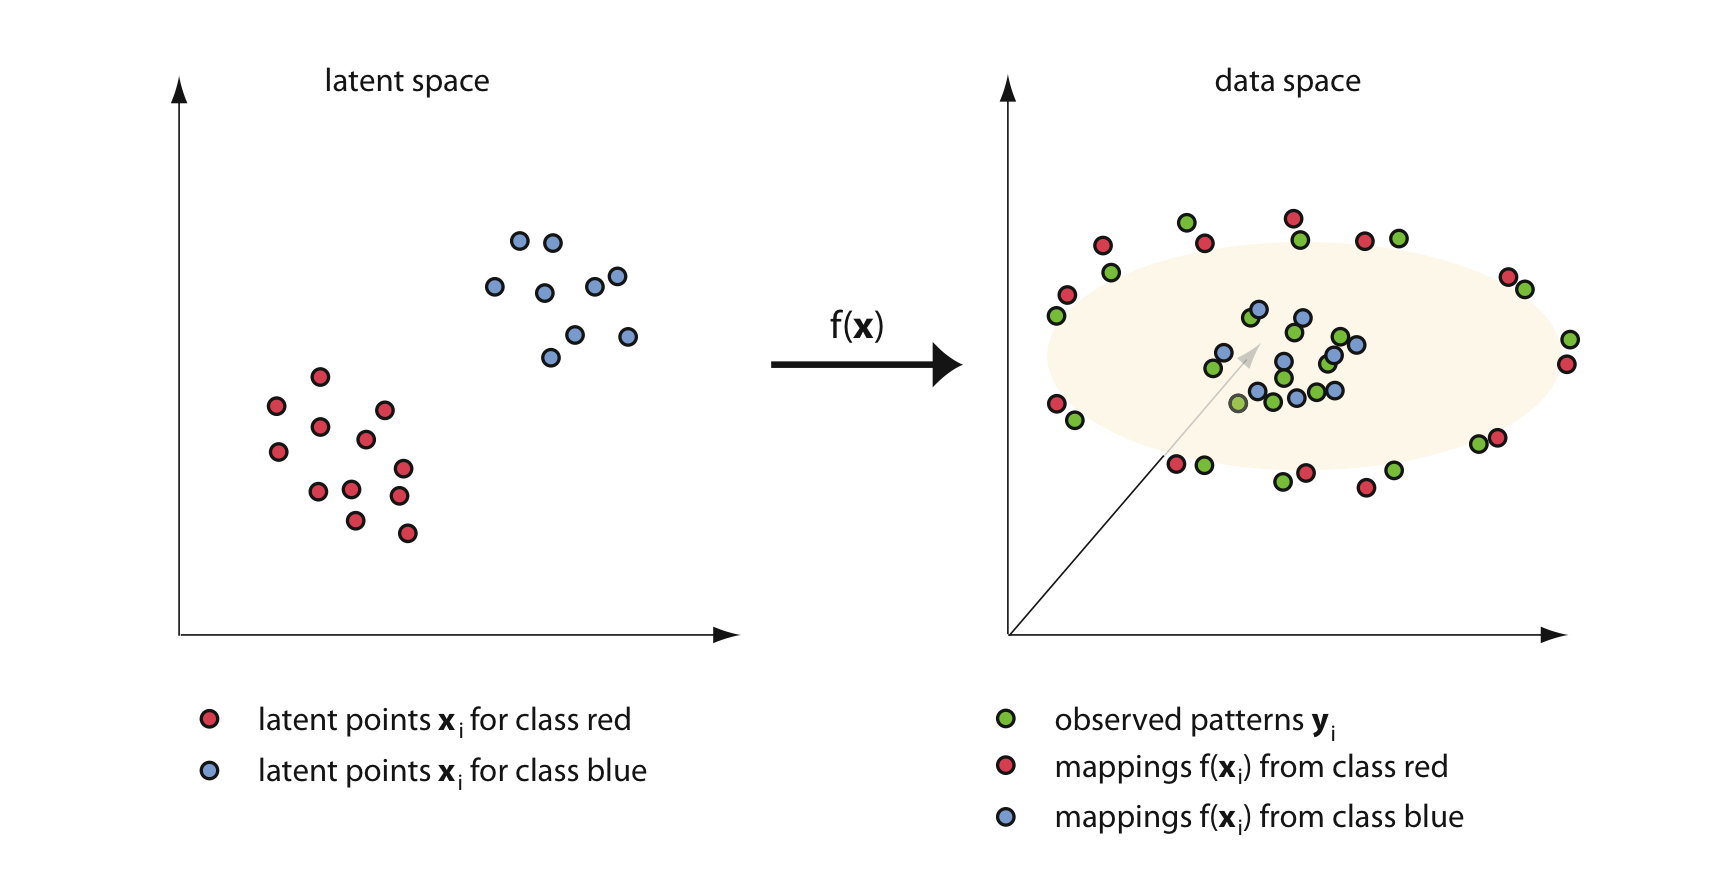
\includegraphics[width=0.9\linewidth]{external_content/graphs/latent_space_reduction_example.png}
  \captionsetup{justification=centering}
  \captionof{figure}{Visual effects from a dimensionality reduction}
  \label{fig:visualisingReduction}
\end{figure}
\todo{This is not my work! This is a placeholder and will be replaced in the final version}

\clearpage
